\chapter{Background Theory and Motivation}
\label{cha:TheoryAndBackground}
This chapter contains the background research and motivation for this thesis.
Section \ref{sec:background} contains the background information regarding swarming and more specifically flocking using the Boids algorithm. How the background research have influenced this thesis can be found in section \ref{sec:motivation}.
%{\it Lorem ipsum dolor sit amet, consectetur adipiscing elit. Nam consequat pulvinar hendrerit. Praesent sit amet elementum ipsum. Praesent id suscipit est. Maecenas gravida pretium magna non interdum. Donec augue felis, rhoncus quis laoreet sed, gravida nec nisi. Fusce iaculis fermentum elit in suscipit.}

\section{Background Theory}
\label{sec:background}
This section will explain swarming and swarm robots. How to implement bird flocking behavior on particles in simulation, and the Boids behavior. It will explain how fish schooling and ant swarm works as well to compliment the bird flocking. Swarms can be used to optimize a problem or they can be used to solve complex problems that would cost a lot more using an advanced robot.
A brief overview of different common robotics architecture will be presented in subsection \ref{sec:robotArch}

\subsection{Swarming}
Swarm, swarming, swarm intelligence, swarm optimization or swarm robotics are terms used for simple (preferably cheap) agents/robots which can only do simple tasks. However, the power of these robots lies in the numbers \citep{Zhu2010,Bonabeau1999}. The robots might not be able to do an advanced task alone, but together they might be able to complete advanced tasks. For instance, one robot might not be able to push a heavy box by itself, but with the help of other robots they might be able to push the box.
The robots are allowed to communicate with each other, but they do not necessarily need to. There is no centralized controller that controls the robot, each one needs to find out what it needs to do by itself or by communicating with the other robots. The idea behind these simple and cheap robots are that they can easily be mass produced, and are interchangeable, modularized and disposable. If one robot is malfunctioning or broken, it would not affect the rest of the swarm. It is therefore no single point of failure in a swarm, and the system scales well because new robots can easily be added to the system.
Swarm robotics are often computational efficient because they each have their own processor. This reduces the computational overhead. 

\subsection{Boids}
In \citep{Reynolds1999}, Craig W. Reynolds created something he called \textbf{Boids}, which stands for \textbf{B}ird-\textbf{oid} object\textbf{s}. Boids are particles that would behave like birds, they would try to flock and fly together without colliding. This was done by using three simple behaviors;
\begin{description}
    \item[Separation]
        Each individual will steer away from the other individual if they are too close to each other. This ensure that they do not collide with their neighbors.
    \item[Alignment]
        In a neighborhood (for instance a radius around the individual or the $X$ nearest individuals) find the average angle of the neighborhood and align itself so its angle matches the average angle of the neighborhood.
    \item[Cohesion]
        Steer towards the average position of the other individuals in your neighborhood. This makes the Boids stay in the flock.
\end{description}

\begin{figure}[h]
    \centering
    \begin{subfigure}[b]{0.3\textwidth}
        \centering
        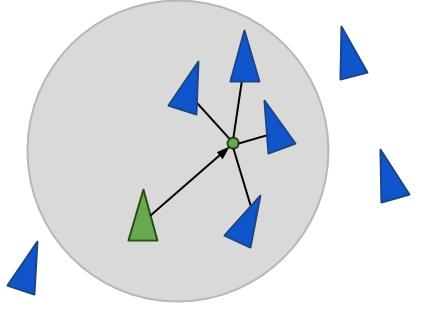
\includegraphics[width=\textwidth]{images/boid_cohesion}
        \caption{Cohesion}
        \label{fig:boid_coh}
    \end{subfigure}
    \hfill
    \begin{subfigure}[b]{0.23\textwidth}
        \centering
        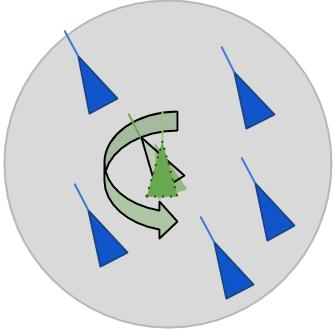
\includegraphics[width=\textwidth]{images/boid_alignment}
        \caption{Alignment}
        \label{fig:boid_ali}
    \end{subfigure}
    \hfill
    \begin{subfigure}[b]{0.3\textwidth}
        \centering
        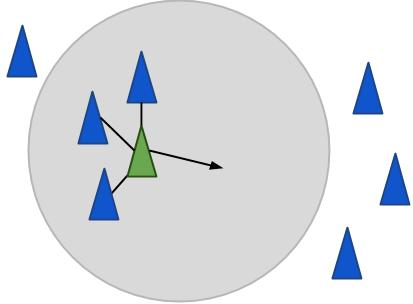
\includegraphics[width=\textwidth]{images/boid_separation}
        \caption{Separation}
        \label{fig:boid_sep}
    \end{subfigure}
    \caption[Boids behavior]{The three behaviors of the Boids \\  based on figures from \cite{1_red3d.com_2015}}
    \label{fig:boidbehavior}
\end{figure}


The three behavior is per individual Boid, which means that each particle/Boid has to calculate where they are going to fly by checking all the other Boids position and rotation and then act accordingly. Which makes the complexity of the algorithm $ O(n^2)$ for every frame. 
Reynolds have tried to make the algorithm less computational expensive by putting the Boids into grids with Spatial Hashing. An example of this could be to put all the Boids that has an $x$-value between 0 and 1 and a $y$-value between 0 and 1 on the lower left grid, and the ones that has an $x$-value between 1 and 2 in the next position etc. Using this grid, each Boids in a cell only needed to take the adjacent grids into consideration when checking their neighborhood. That way they do not need to check the position and rotation of all the other Boids.
\begin{figure}[h!]
    \centering
    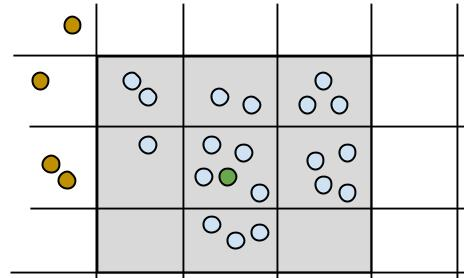
\includegraphics[width=0.8\linewidth]{images/boid_spatialhash}
    \caption{Boids in grids using spatial hash} \label{fig:spatialhash}
\end{figure}
As illustrated in figure \ref{fig:spatialhash}, the green Boid only needs to check the gray Boids that surrounds its own cell, it does not need to check the rotation and position of the orange/brown Boids outside of the gray highlighted area, because they are too far away to be considered a part of its neighborhood.

In another paper \citep{Joselli2009} a different technique were used to optimize 3D swarms, a method using neighborhood grids.

Each Boids to cell ratio would be 1 to 1, that is for every cell, there would be at max 1 Boid. Each Boid would have their respective cell based on their position in space, for instance a Boid with low $x$-value would be on the left of a Boid with higher $x$-value. Boids who are closer to each other in geometric space would be stored closer to each other in the grid. To obtain this, the Boids needs to be sorted. Odd Even sort and Bitonic sort were used as the sorting algorithm. See appendix \ref{app:sorting} for more detail.

Of the two sorting algorithm, Odd Even sort was faster, but not very precise. More than 10\% of the entities were placed in the wrong cell. An Odd Even sort algorithm had to be done for each axis, that is one odd even sort for x, y and z. Each axis were sorted in parallel.
Bitonic Sort on the other hand was slower, but a lot more precise. Less than 1\% of the entities were placed in wrong cell. The reason for placing a Boid in the wrong cell is due to the way the sorting works, it sorts all the entities in one axis first, then a second axis and then the third last axis. For instance sorting on $x$-values first, for the $y$-values, then the $z$-values. When swapping one of the latter axises it might mess up the sorting of one of the other axises.

After the Boids were placed in their corresponding cell, the work could be distributed to the GPU which would calculate where each Boids' new location and rotation would be based on their adjacent neighbor depending on the Moore radius. A Moore radius of 2 would cover the current square, the adjacent squares and their adjacent neighbors as well. The Moore radius is used to determine how many other Boids to consider in its neighborhood. For instance if the Moore radius is 2, the Boids will have a neighborhood as illustrated by the gray color in figure \ref{fig:moore}. Each cell is supposed to contain a Boid.
\begin{figure}[H]
    \centering
    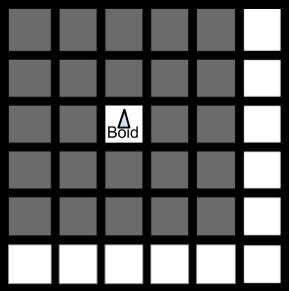
\includegraphics[width=0.3\linewidth]{images/moore}
    \caption[Moore radius illustrated, 2D]{A Moore radius of 2 illustrated by the gray squares \\ based on the figure from the paper \citep{Joselli2009}}\label{fig:moore}
\end{figure}
In 3D space, extra layers would be added. A Moore radius of 1 would cover all the adjacent grids, which would make the 8 grids that we have in 2D space plus 9 grids above and 9 grids below. That would equal 26 grids, compared to the 8 squares in 2D space. A Moore radius of 2 would cover 74 grids in 3D space (24 + 25 above and 25 below). See figure \ref{fig:3dgrid} for an illustration of the space covered by a Moore radius of 1 in 3D space, this illustration is only an intersection and does not show all the covered grids.
\begin{figure}[H]
    \centering
    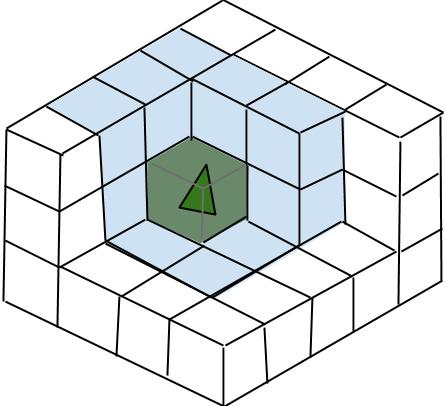
\includegraphics[width=0.5\linewidth]{images/3dgrid}
    \caption[Moore radius illustrated in 3D space]{An intersection of a Moore radius of 1 in 3D space \\ based on the figure from the paper \citep{Joselli2009}}\label{fig:3dgrid}
\end{figure}

The number of Boids was varied from 1,000 to 1,000,000 and the number of Boid types was varied from 1 to 4. Boids of the same type would try to flock with each other while different types of Boids would try to avoid each other.
They were able to see a speedup compared to the spatial hashing method used by Reynolds, but the Boids were not rendered as a bird or an object, only as a primitive shape. They didn't mention if they tried to add non moving obstacles in their test. Due to the high percentage of Boids being placed in the wrong cell when using odd even sort, a lot of Boids would crash into their neighbor during the test run. However using the neighborhood grid method on GPU, real time simulation of 1 million Boids were possible (6-8 fps).

In the paper "steering behaviors for autonomous character" Reynold discusses steering for autonomous character in games and animation, which is a type of autonomous agent that have some ability to improvise their actions. That means that these agents do not have their actions scripted in advance.
It is possible for the Boids to have more behaviors, called steering behaviors as explained in \citep{Reynolds1999}. The steering behavior decides where the Boids are supposed to steer after their three simple behavior are satisfied.  These steering behavior can be seek, flee, pursuit, evade etc. 

%The \textbf{seek} behavior tells the Boid to seek a goal, it will try to reach the goal/object as fast as possible, and due to the high speed it has when arriving it will fly past the goal. It then turns around to seek the goal again.
%A seek behavior should have an \textbf{arrival} behavior to counteract the fly-by, that means that when nearing the goal, the Boid will slow down so it stops at the goal in the end, instead of flying past it.
%
%A \textbf{flee behavior} is almost the same as the seek, except in the opposite direction. It will try to turn away from the "goal" and fly in the opposite direction or rather fly as far away from the "goal" as possible.
%
%\textbf{Pursuit} is the same as seek, except it applies to moving objects. Pursuit requires prediction of the target's future position. The approach is to predict the future position of the target, reevaluate and readjust it each step. A prediction might be wrong at one time step, but this only applies for that single time step, and a new prediction will be made at the next time step which hopefully will be correct.
%
%An \textbf{offset pursuit} behavior behaves almost the same way as the normal pursuit behavior, except that it will not "crash" into the target but have an offset or $R$. An example of this could be an aircraft flying near the sensors of a base or something similar. 
%
%\textbf{Wander} behavior is a type of random steering, the particle move randomly around, An easy way to implement this behavior is to apply a random steering force each frame, but this leads to twitchy movements, which doesn't look very natural. The proposed method is to have a steering direction which is being displaced each frame with a very small random force.
%That way, if the particle is move forward, it will still keep moving forward the next frame, but it might turn a little bit to the right. Which makes it seem a lot more natural.
%
%\textbf{Path following} behavior enables, as the name suggest, a character to follow a predefined path. However it is not as strict as a train following the rail tracks, the character are allowed to deviate a little bit from the track. The implementation involves a spine with a radius, which makes the track. The path makes a tube in 3D or a thick line in 2D. The goal for the path following behavior is to first reach the tube, then stay inside this tube, thus following the path. Variations of path following are wall following, and containment. Wall following ensures that the character followes the wall, while containment refers to motion restricted inside a region.
%
%\textbf{Leader following} behavior makes one character follow another character. The follower wants to stay near the leader, but also stay out of the way. If there is more than one leader, they also want to avoid bumping into each other. The implementation of leader following behavior relies on the arrival behavior where the goal is a point behind the leader. The follower will slow down when drawing near the point behind the leader and eventually stop before it bumps into the leader. If the entity is in front of the leader, it will fly away and around the leader so it is not in the way.
\begin{description}
\label{boids:behaviors}
\item[The seek]behavior tells the Boid to seek a goal, it will try to reach the goal/object as fast as possible, but due to its high speed it might have when arriving at the goal, it will fly past the goal. It will then turn around to seek its goal again.

A seek behavior should have an \textbf{arrival} behavior to counteract the fly-by, that means that when nearing the goal, the Boid will slow down so it stops at the goal in the end, instead of flying past it.

\item [Flee behavior] is almost the same as the seek, except in the opposite direction. It will try to turn away from the "goal" and fly in the opposite direction and fly as far away from the "goal" as possible.

\item [Pursuit] is the same as seek, except it applies to moving objects. Pursuit requires prediction of the target's future position. The approach is to predict the future position of the target, reevaluate and readjust it each step. A prediction might be wrong at one time step, but this only applies for that single time step, and a new prediction will be made at the next time step which will hopefully be correct.

\item [Offset pursuit] behavior behaves almost the same way as the normal pursuit behavior, except that it will not "crash" into the target, but will have an offset $R$. An example of this could be an aircraft flying near the sensors of a base or something similar. 

\item [Wander] behavior is a type of random steering, where the particle moves randomly around. An easy way to implement this behavior is to apply a random steering force each frame. But this leads to twitchy movements, which does not look very natural. The proposed method is to have a steering direction which is being displaced each frame with a very small random force.
That way, if the particle is move forward, it will still keep moving forward the next frame, but it might turn a little bit to the right. Which makes it seem a lot more natural.

\item [Path following] behavior enables, as the name suggest, a character to follow a predefined path. However it is not as strict as a train following the rail tracks, as the character is allowed to deviate a little bit from the track. The implementation involves a spine with a radius, which makes the track. The path makes a tube in 3D or a thick line in 2D. The goal for the path following behavior is to first reach the tube, then stay inside this tube, thus following the path. Variations of path following are wall following, and containment. Wall following ensures that the character follows the wall, while containment refers to motion restricted inside a region.

\item [Leader following] behavior makes one character follow another character. The follower wants to stay near the leader, but also stay out of the way. If there is more than one leader, they also want to avoid bumping into each other. The implementation of leader following behavior relies on the arrival behavior where the goal is a point behind the leader. The follower will slow down when drawing near the point behind the leader and eventually stop before it bumps into the leader. If the entity is in front of the leader, it will fly away and around the leader so it is not in the way.
\end{description}

\subsection{Collision Avoidance}
In the paper \citep{CraigW.Reynolds}, W. Reynolds discusses how to perform obstacle avoidance. That is, obstacles that are placed in the environment which is not a Boid. These obstacles are usually static, non moving obstacles. He starts out with the idea of a force field around the obstacle which he calls the \textit{steer away from surface} approach. The idea is to have every obstacle emit a forcefield around itself which pushed the Boids away. For instance if a Boid is flying toward an obstacle, the obstacle would push the Boid to one side of itself. However this force field method would not work if the Boid flew straight into an obstacle, because the forcefield force would be straight opposite of the direction the Boid is flying thus making the Boid decelerate until it stopped.

The next obstacle avoidance technique Reynold discussed is the curb feeler technique or steer along the wall technique. The idea is to have a feeler that would detect an obstacle before the Boid would crash into it, then turn the Boid away from the obstacle. This can be compared to walking down a dark alleyway where you reach your hand out to feel the walls around you, and navigate through the alleyway just by feeling the wall(s).

The last technique for navigating and avoiding obstacles discussed was image processing. Images could be processed in real time to a gray scale image, where white would signify an obstacle. The algorithm would start with the center of the image, if this was a white pixel it would start to search outwards in a spiral to find either a gray pixel or a black one and then turn the Boid in this direction. This could also be combined with a \textit{Z-buffer image} which gives us a map of the distances to obstacles that lies in front of the Boid, this z-buffer image can be obtained by radar, sonar or similar technology. One interesting way of using the Z-buffer image is to implement a "steer towards the longest clear path". However using this technique without any form of planning or learning might lead the Boid into a local cavity, which might be a dead end.

\subsection{Physic based control system}
In the paper \citep{Spears2004}, a self emergent system was formed using simple attractive and repulsion force for each particle. The idea behind their system was to create an artificial physics framework (AP) that would simulate a physical system. In their paper they had the particles attract other particles that were farther away than distance \textit{r} and a repulsive force is applied if the particles are closer than distance \textit{r}. This leads to the particles always being at distance \textit{r} from each other, which will form a hexagonal lattice. In the hexagonal lattice, each particle will be at a distance $r$ away from each other, but the next neighbor will be $\sqrt{3}r$ away. Therefore each particle only have a vision range of $1.5r$ so they do not affect the particles that are too far away from it. 

In the simulation they spawned all the particles in a cluster, using the two-dimensional Gaussian random variable to initialize the position of the particles. The particles starts with a velocity of 0.0, but their framework does not require so. Due to local forces, the particles will disperse and form local hexagons. To evaluate the quality of the lattice they measured the orientation error of the lattice: they took any particles that were $2r$ apart and formed a line segment, then they took any other particles that were $2r$ apart and formed another line segment. The angle between these to line segments should be measured to be a multiple of $60^{\circ}$. The error would be the absolute value of the difference between the measured angle and the nearest multiple of $60^{\circ}$. The error ranges from $0^{\circ}$ to $30^{\circ}$.

They also checked the size of the particle cluster. For each particle $i$ they counted the number of "close" particles, that is particles that are in the range of $0<r<0.2r$. The minimum cluster size is 1.0 because they count the particle $i$ as well as its neighbors. The cluster count was averaged for all the particles. At the start there was a high cluster count, but it decreased to roughly 2.5 after 6 time steps. 

They also tried out making square patterns, but had to introduce a concept of spin; each particle was either spin "down" or spin "up". Opposite spins would attract each other if the distance was greater than \textit{r}, and repel each other if the distance is less than \textit{r}. If the particles had opposite spin the distance would be $\sqrt{2}r$. This means that all the particles on the vertical space would be alternating between spin up and spin down, the same goes for the particles in the horizontal space. The particles on the diagonal will have the same spins as their diagonal neighbors. Sometimes the formation would have "holes" in it, so instead of static spins, the particles were allowed to change their spin. This would fill in the holes or flaws in the square lattice, according to their theory.

A particle would only change its spin if it had a very close neighbor ($r<1$), and the probability of changing spin was quite small.

\subsection{V like bird formation}
In the paper \citep{Nathan2008}, bird flocking is discussed, they wanted to simulate the V shape that can be observed when birds fly together. They ran a simulation that where each bird individual had three simple rules: 
\begin{itemize}
    \item \textbf{Coalescing rule}: \\
        The birds should try to seek the proximity of the nearest bird.
    \item \textbf{Gap-seeking rule}: \\
        If rule 1, the coalescing rule is not applicable anymore the bird should find a position with unobstructed view -  that is, the bird should be able to see in front of it without anything being in the way.
    \item \textbf{Stationing rule}: \\
        Try to stay in place.
\end{itemize}
These rules would make sure that the birds were able to flock and form different shapes. The only thing that was common between the different runs in this paper was that the bird behind would be a little bit behind and slightly left or right of the bird in front (following rule \#2). A lot of different shapes was obtained during the runs, the birds flocked and formed a V-shape, a diagonal line, an inverted V-shape etc.

\subsection{Family bird: A heterogeneous simulated flock}
The paper \citep{Demsar2013} by \citeauthor{Demsar2013} says that bird flocks and fish schools seems to be very complex, but the mechanics are very simple as illustrated by Reynold. Only a few simple rules will create flocks that flock together and splits up to avoid obstacles. These flocks are not spectacular or mind blowing compared to the flocks found in nature, due to the rigid motion of each individual. To tackle the artificialness of each individual, Heppner introduced randomness to the motion of the individuals. He defends it by saying that these randomness simulates wind gust, random obstacles and other factors. 
However, the authors of this paper does not agree with this approach because wind gusts will affect the whole flock, not just a random single individual at random. Even with these randomness added, the flock still does not seem lifelike enough compared to their counterpart found in nature. The reason for the lack of breathtaking in these flocking algorithms are that the individuals all have the same characteristics. In nature each individual will have different size, age, form and shape.
 
Usually in flocking algorithms, each individual takes into account where all the other entities are and then act accordingly. In nature, each individual might have limited information about the flock. It might only be able to gain so much from its vision due to other flock members being occluded or not able to hear some of the other individuals due to noise or other factors.

This paper runs a simulation with different types of birds, where social relations are a factor and individuals might be solitary or social. Social individuals are entities who would like to stay close to members of its own social group, for instance a social dove will want to stay with other doves. Solitary individuals on the other hand does not care about staying with its own flock and might drift to another flock. For instance a solitary dove might fly amongst hawks or other types of birds. A flock in this paper are defined as a group where the individuals affect each other in the same group. The simulation they ran varied between all solitary birds to 4 types of different social birds.

\subsection{Particle Swarm Optimization}
Swarms has a lot of potential, not necessary only on robotics but swarms can be used to optimize problem, hence the name \textbf{particle swarm optimization (PSO)} \citep{Eberhart}. PSOs is used to solve problems where optimization are needed. The idea behind PSOs are to have a swarm of particles spawn at random positions in the search space, and then let them fly around searching for solutions. Each particle will know the best solution it have found so far, and the best solution that has been found globally. In some PSO implementations a local best found solution is also known amongst the individual. This local best solution is the best solution amongst a subgroup of individuals and can change for a particle depending on the position of the particle. 

If all of the particles were to be attracted to only the global best found solution so far, they might risk to be stuck in a local maxima without being able to find the other local maximas. To avoid being stuck in a local maxima, each particle is also attracted to the best solution it has found, and maybe to the neighborhood's best found solution as well. This ensure that the particles "jiggles" (introduces enough noise) so that the particle might jump to another local maxima. 

\subsection{Other swarming animals}
This section will look at other flocking animals or insects and how they have been modeled in simulation.
\subsubsection{Fish schools}
In the paper named "Artificial Fishes: Autonomous Locomotion, Perception, Behavior, and Learning in a Simulated Physical World" \citep{Demetri1994} we are given the explanation on how fishes form schools and how different intentions make the fish behave the way they do. He starts out with explaining how a fish and how the simulator is constructed, the math behind it and how the motor controllers work. For the simulation there is different types of fishes, some of them are predators and some of them are preys. Where predators are larger fishes which tries to eat other smaller preys. Each fish has a 300 degrees, where it can see in front of it and has a blind spot directly behind it. These fish uses the containment behavior mentioned earlier, where they swim freely around in the aquarium, but are not allowed to/not able to leave it.

The range of the vision is also limited and might be occluded by other objects. Each fish has a intention generator, which basically is a flowchart of what the fish needs to do. The prey and predator fish have different intention generators. The predators do not get preyed upon, and thus does not need to look out for other predators, therefore are the intentions of escaping, mating and schooling with other fishes of the same species are disabled. The reason for disabling mating is because there is no need for new predator fishes because they do not die in this simulation. They also do not need to school with other predators because they are not in danger, and do not need the extra survivability.

Whenever a predator sees a prey it will chase the prey if the cost of reaching it is low enough. If it is too high, it will not bother chasing.

Preys on the hand needs the extra survivability, and will try to school with the other fishes if it detects a predator nearby. Each fish will then try to stay a certain distance from the others, which is roughly one body length in distance. Then the fishes will try to adjust its speed and direction so it matches the other members. When this school of fish encounter an obstacle, each individual fish will try to avoid this obstacle. This might lead to the school splitting up and rejoining after they have avoided the obstacle.

A third type of fish introduced here are the pacifists fish. This one differs from the other two type in that the intention of mating is activated while escaping and schooling are deactivated.
The paper describes that there are male and female fishes, and the two behavior which can occur when the fishes start to mate. A behavior named \textit{nuzzling} where the male fish seeks the female and nudges her abdomen until she's ready to spawn, and \textit{spawning ascent} where the female swims repeatedly to the surface while releases gametes. The paper also describes in detail how the fishes select potential partners and how they try to impress each other for mating purposes.

\subsubsection{Ant swarms/colonies}
Ant swarms behaves differently than other types of swarms \citep{Blum2005}, ants do not try to form formations for survival in the same way that birds and fishes do. Ant swarming is mostly about their foraging behavior. That is how they find food for their colony. Each ant's goal is the survival of the colony rather than the survival of each individual. When ants try to find food, they scatter the area by walking in random manner. While exploring the ants leave behind a chemical on the ground. A so called pheromone that the other ants will be able to feel/smell. This pheromone will slowly but surely dissipate. Whenever the explorer ant find a food source, it will evaluate the quality of the food before returning to the anthill. During the return trip, pheromones are reapplied to the path, but the amount is adjusted based on the evaluation of the food. Better food will yield more pheromone on the path. This method will ensure that the rest of the ants will take the shortest path from the anthill to the food. For the artificial ants, the ant system uses a graph $G = (V,E)$ to model the paths, $V$ are the nodes and $E$ are the edges between the nodes. In the paper \citep{Blum2005}, they use two nodes: $v_s$ which is the starting node or anthill. The node $v_d$ is the food source. There is two ways to reach the food source from the anthill, $e_1$ and $e_2$, which have lengths $l_1$ and $l_2$ where $l_2 > l_1$. A value $\tau_i$ denoted the artificial pheromone, and it indicates the strength of the pheromone. 

An ant will choose a path with the probability $p_i = \frac{\tau_i}{\sum_{ n = 1}^{k}\tau_n}$ where $k$ denotes the number of paths. In the paper, they only have two paths, so the probability of choosing a path is $p_i = \frac{\tau_i}{\tau_1 + \tau_2}, i = 1,2$.
The ant will probably choose $e_1$ if $\tau_1 > \tau_2$ and vice versa.
The ants will return using the same path as the one it took, and reinforce the path with new pheromones using the formula $\tau_i \leftarrow \tau_i + \frac{Q}{l_i}$ where $Q$ is a positive constant. The pheromones that have already been laid out in the path will slowly evaporate, the evaporation formula used is $\tau_i \leftarrow (1-\rho)\cdot\tau_i, i = 1,2$, where $\rho \in (0,1]$. These math formulas will over time make sure that the ants are converging to the short path.

The biggest difference between these artificial ants and real ones are that these move synchronously, while real ants are asynchronous. Real ants leaves pheromones on the ground whenever they move, these artificial ones only leave behind the pheromones on the way back to the anthill. The normal ants' pheromone strength are due to evaporation, while the artificial ones regulates the strength of the pheromones using an evaluation of some quality measure. The ant system can be used for approximate algorithms for combinatorial optimization problem, especially for combinatorial problems which are NP-hard.

\subsection{Robot architectures}
\label{sec:robotArch}
Software architecture is the methodology for structuring the code or algorithm. One software architecture model might work better for one purpose while another architecture works better for a different purpose. 

\begin{figure}[H]
    \centering
    \begin{subfigure}[b]{0.25\textwidth}
        \centering
        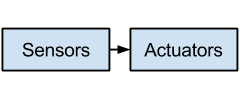
\includegraphics[width=\textwidth]{figs/reactive}
        \caption{reactive control architecture}
        \label{fig:reactive}
    \end{subfigure}
    \hfill
    \begin{subfigure}[b]{0.4\textwidth}
        \centering
        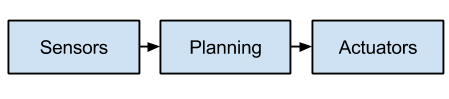
\includegraphics[width=\textwidth]{figs/deliberative}
        \caption{deliberative control architecture}
        \label{fig:deliberative}
    \end{subfigure}
    \hfill
    \begin{subfigure}[b]{0.3\textwidth}
        \centering
        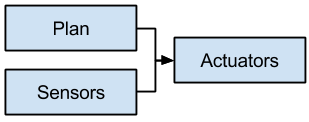
\includegraphics[width=\textwidth]{figs/hybrid}
        \caption{hybrid control architecture}
        \label{fig:hybrid}
    \end{subfigure}
    \caption[Robot architecture]{Robot control architectures}
    \label{fig:robotArchitectures}
\end{figure}

This subsection will briefly explain common architectures found in robotics. In robotics, the architectures needs to decide how to combine reactive control and model-based deliberative planning. Reactive robots relies mostly on their sensor inputs and reacts accordingly. For example a robot equipped with distance sensors that usually drive forward might turn if the front distance sensor detects an obstacle.

Deliberative planning on the other hand also uses the available sensors on the robot, but they do not react immediately like the reactive robots would do. Deliberative planning robots uses the information gathered from the sensor(s) to make a plan of where it should head or what it should do, before executing its action(s).

A mix of both planning and reactive robot architecture which uses reactive techniques at lower level and deliberative planning at the higher levels are called hybrid architectures.

\subsubsection{Brooks subsumption}
\label{sec:brooks}
Brooks subsumption architecture is the most common reactive robot architecture. As explained earlier, a reactive architecture is based on a direct sensor to actuator mapping. That is, whenever a sensor measures anything over a predefined threshold or if the sensor senses anything, the actuator will react immediately. The idea behind the subsumption architecture is to split the behavior of the robot into sub-behaviors into a vertical hierarchy as illustrated in figure \ref{fig:subsumption}. 
\begin{figure}[H]
    \centering
    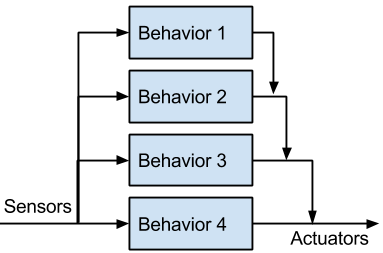
\includegraphics[width=0.5\linewidth]{figs/subsumption}
    \caption[Subsumption architecture]{Subsumption architecture}\label{fig:subsumption}
\end{figure}

As seen in the figure, the sensors input the information it have sensed, and each behavior reacts accordingly. A higher level of behavior will have higher priority than the lower ones. For example, behavior 4 in figure \ref{fig:subsumption} would have priority over behavior 3, and behavior 3 would have priority over behavior 2 etc.


The advantage of the Brooks subsumption architecture is that the robot using it can have different goal depending on the specific situation. For example, if you have a robot that needs to find a specific item in an area. This robot would first wander around aimlessly, and its sensors would be used to avoid crashing into obstacles or other robots. When the robot has located the item it wants, it would use its sensors to move towards that item instead of using it to avoid it, its sensors could be used to align itself with the item to push it towards a different location.

\subsection{Deliberative control architecture}
Deliberative control architecture are based on Sense-Plan-Act principle as seen in figure \ref{fig:deliberative}, the robots uses its sensors to get a full overview of the environment. After it have gained full knowledge of the environment, it will plan solutions then consider them before choosing an action. Deliberative planning robots are usually very dependent on precise sensors to be able to map the environment. It is also assumed that the model of the world the robot will be in is provided. 

\subsubsection{Hybrid control architecture}
\label{sec:hybrid}
Hybrid architecture is a mix of deliberative control architecture and reactive architecture. The idea behind the hybrid control architecture is to work around the limitation and drawbacks of both the reactive and the deliberative control architecture.

\begin{figure}[H]
    \centering
    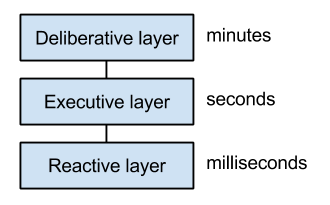
\includegraphics[width=0.5\linewidth]{figs/threelayer}
    \caption[Three layer architecture]{Three layer control architecture}
    \label{fig:threelayer}
\end{figure}

The hybrid control architecture usually have a deliberative layer to plan and model the environment, but the deliberative controls might be slow and not able to act fast enough in certain situations. Each decision might take minutes. The environment that the deliberative layer creates or maps out can be learned from data or gathered through the sensors from the reactive layer.

That is why the reactive layer is added to the control architecture as well. The reactive layer usually have faster reaction time than the deliberate layer, and can help the robot navigate when they need to do an action fast. The reactive layer's decision cycle is often on the order of milliseconds.

To glue together the reactive layer and the deliberative layer, a layer is put in between the lower reactive layer and higher deliberative layer. Namely the executive layer or sequencing layer. The executive layer accepts directive from the deliberative layer and puts them in order for the reactive layer. The executive layer is slower than the reactive layer, it takes seconds to make a decision.

The hybrid architecture explained here is the most common architecture for the hybrid control architecture, which is called the three-layer architecture due to the three layers deliberative, executive and the reactive layer as seen in figure \ref{fig:threelayer}.

%Kan nevne andre systemer som har implementert Boids 

\subsection{Related systems and projects}
\label{sec:relsys}
This subsection will look at systems and projects where the flocking algorithm have been implemented on a physical robot.

\subsubsection{Flocking on wheeled robots}
In 1992, Matari\'{c} designed a series of behavior based modules for mobile robots, that would make them flock if combined and properly weighted. The wheeled robot were equipped with collision sensors, and six distance sensors. By using these sensors combined, the robots would be able to measure the distance to the other robots within a small neighborhood. Matari\'c implementation uses four behaviors;
\begin{description}
\item[collision avoidance] makes the robot steer away from objects that are closer than a predefined
\item [following] makes the robots follow the other robots, this behavior is implemented by using the two sensors on its side. If there is only one perceived object on either side of the robot, it will turn towards that side. If there are other robots on both its side, it will keep moving forward along with the other ones until there is a robot in front of it blocking its path.
\item[Dispersion and aggregation] Steers the robot towards the computed center of mass, this center of mass is computed using the reading from the sensors.
\end{description}
This system uses five robots with the subsumption architecture. The space the robots are empty, that is no obstacle or walls. If these robots were to flock through a cluttered environment, a more sophisticated sensing ability would be required. There were other behaviors implemented on these robots as well, but the four behaviors mentioned above are the ones that makes the robot flock.

\subsubsection{Flocking on quadcopters}
In the paper \citep{Csaba2014} a flocking algorithm were implemented on quadcopters. Ten of these quadcopters were flying around in the air autonomously, they would communicate with each other and all of these quadcopters had access to a GPS.
The swarm could form shapes, for example forming circles or lines when instructed to do so. When forming a circle, each quadcopter had to take its place on the circle by evenly spacing themselves on the perimeter of the circle. The quadcopters were also able to do leader following behavior.
The implementation uses GPS to determine the position of the quadcopters, but their algorithm works with all other sensory input where relative position, velocity and altitude information can be obtained. Their swarm flock were dependent on sensory errors and delays in the system. The researchers were able to fly this swarm flock of quadcopters for 20 minutes.

The algorithm were implemented in two and a half dimension, that is the quadcopters would fly up to the correct altitude, and the flocking and formation part of the algorithm would only work in two-dimension after the copters had reached its correct altitude. Each of the quadcopters had to have a 6-10 meters between them due to inaccuracy from the GPS and other disturbances found in the air. If they were to flock at closer than the 6-10 meters range, they would risk crashing into each other.

%\section{Structured Literature Review Protocol}
%TODO
%Key words used:
%Swarm
%robotics
%two wheeled differential drive
%Boids
%Birds Flocking
%Fish School
%Ant


%Here you need to include your structured review protocol including search engine, search words, research questions  (for search, not the masters research questions), inclusion createrias and evaluation Criterias. 

\section{Motivation}
\label{sec:motivation}
Most of the flocking systems mentioned in this chapter makes the entities flock together by using some sort of attracting force, and when they are too close to each other, a repellent force acts upon the entities to keep them at a fixed distance from each other.
Swarming is an emergent field in artificial intelligence, nowadays it is becoming more popular with more smaller robot than one expensive traditional robot, especially when it comes to AI research. There are some few other projects where flocking behavior has been implemented as mentioned in section \ref{sec:relsys}, one of the project used moving robots but had advanced sensors that were able to differentiate between the robot and other objects. The second project mentioned used flying quadcopters that flew in two and a half dimension. The latter one used GPS to the quadcopters so they would know where in the space they were positioned. However they had to have a pretty big gap between them to be sure that they did not crash into each other.
There are various applications for flocking robots, some of them are mentioned in \citep{Csaba}. Flocking robots can be used for surveillance if they are equipped with cameras, search and rescue operations. A swarm of flocking robots could fly over a farm to check the health of the soil or the vegetables that are grown there. 
% and to get a better understanding of how swarming and flocking works

In this thesis the Boids algorithm will be used to make the ChIRP robots move together in a flock. A centralized computer will help aid them, by acting as a communication bridge between the robots, and by using the camera it will also act as a GPS. By using distance sensors, the robots might be able to move close to the other robots without crashing, and the centralized computer might help make the robots gain information about its surrounding.

%Help CRAB lab further develop the ChIRP robot.



%Your motivation can be either application driven or technique/methodology driven. However in both cases, there will be an element of methodology driven due to the research focus of our group and the nature of a masters project.  
%What other research has been conducted in this area and how is it related to your work? The text should clearly illustrate why your goals and research questions are important to address. This section is thus where your literate review will be presented. It is important when presenting the review that you present an overview of the motivating elements of the work going on in your field and how these relate to your proposal, rather than a list of contributors and what they have done. This means that you need to extract the key important factors for your work and discuss how others have addressed each of these factors and what the advantages/disadvantages are with such approaches. As you mention other authors, you should reference their work. Note that the reference list reflects the literature you have read and have cited. This will only be a subset of the literature that you have read. 